\documentclass[a4paper,12pt]{IEEEtran}
\usepackage{graphicx}
\usepackage[greek,english]{babel}
\graphicspath{{./report_plots/}}
\begin{document}

\title{CSC 510 Assignment 2 Report}
\author{Justin Oakley}
\maketitle\

\pagenumbering{arabic}
\tableofcontents
\newpage

\section{Introduction}
This report is about knowing machine learning techniques that will help in selecting suitable techniques which will provide excellent quality results for applications using the computing environment utilized in an experiment. The reason for why understanding these methods are so important in big data is because they provide higher quality data not only for machines to processes, but also for them to produce. The steps taken in order to obtain the desired data output are based on the type of learning that the machine must go through and the appropriate selection of models and algorithms that follow with that type of learning. In this assignment, supervised learning is the main type of learning that will be focused upon and the modeling strategies that will be heavily utilized in data analyzation are regression and classification.

As for the information that was processed, five different datasets were used in this assignment; one computer-generated dataset of fifty observations alongside two datasets based on recent graduate and graduate students, called \textit{recent-grads.csv} and \textit{grad-students.csv}, are experimented on in the regression model section, and two datasets about captured network normal and attack traffic, named \textit{nslkdd-version1.csv} and \textit{nslkdd-version2.csv}, are utilized in the classification portion. All data analyzation for the assignment is coded in the Python 3 language via the Apache Spark 2.4.0 computational engine on an Apache Hadoop cluster. With this in mind, the goal of the comprehending supervised machine learning techniques through model and algorithm selection can be achieved.

\section{Comparison of Regression Models}
The first step in developing a working knowledge of the functionality of machine learning techniques is to understand the significance of regression. Regression modeling is about predicting values based on the actual responses of \textit{y} and the domain values of \textit{x} being utilized in the processes of an error factor minimization and regularization to paramterize the model:  \[\textit{y} = \textit{A}\textbf{x}' - \textit{b}\] In order to accurately predict values using regression, the optimization process must take place, which means that several different models must be parametrized and compared together to see which has the lower error factor.

For this experiment, four different types of regression were performed on a generated dataset of fifty observations and the \textit{recent-grads.csv} and \textit{grad-students.csv} files. The three datasets where processed through all four types of regression to find the optimal parameters needed to make the most accurate predictions and the best fitting line or hyperplane. The four regression models used in this portion of the assignment were standard regression, ridge regression, lasso regression, and elastic-net regression. In the following subsections, each dataset's regression models will be compared and contrasted together, respectively.

\subsection{Generated Set of Points}
\label{gen_set}
In standard regression, the estimated parameter is found by calculating: \[\textit{A} = \textit{y}\textbf{x}'(\textbf{x}\textbf{x}')^{-1}\] then plugging the matrix \textit{A} into the model equation. When using the one-dimensional domain formed by the generated set of points was applied this algorithm, the following figure spawned: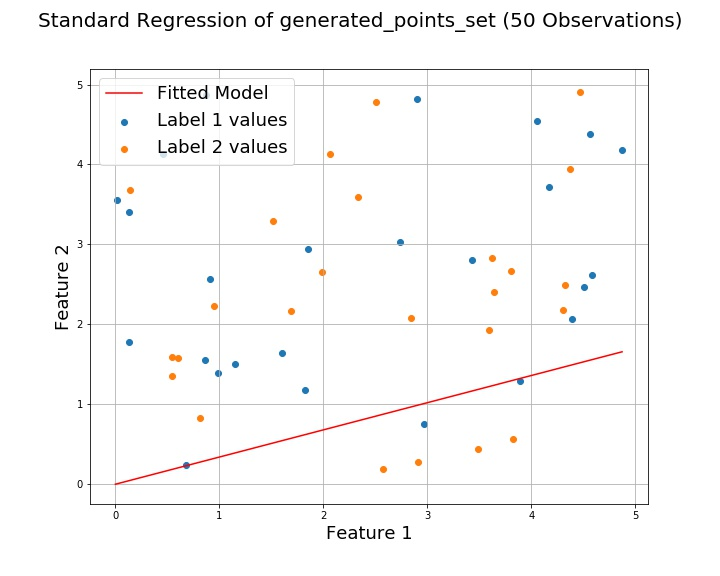
\includegraphics[width=8cm]{std_reg_1d_generated_points_set} while the two-dimensional domain of the dataset resulted in: 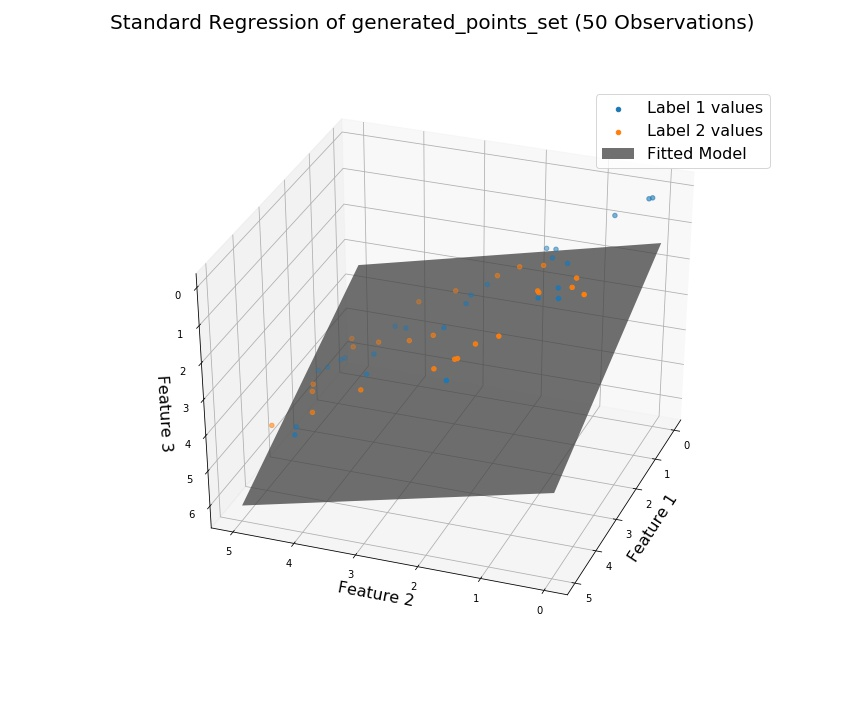
\includegraphics[width=9cm]{std_reg_2d_generated_points_set}

Now in the processing of the ridge regression model, where the regularixation parameter is $\lambda \textit{a}^{2}$ which gives the estimate for the vector (matrix) model is
$$\textit{A} = \textit{y}\textbf{x}'(\textbf{x}\textbf{x}' + \lambda \textit{I})^{-1}$$the following plots were created from one-dimensional domain and the two-dimensional domain of the dataset: 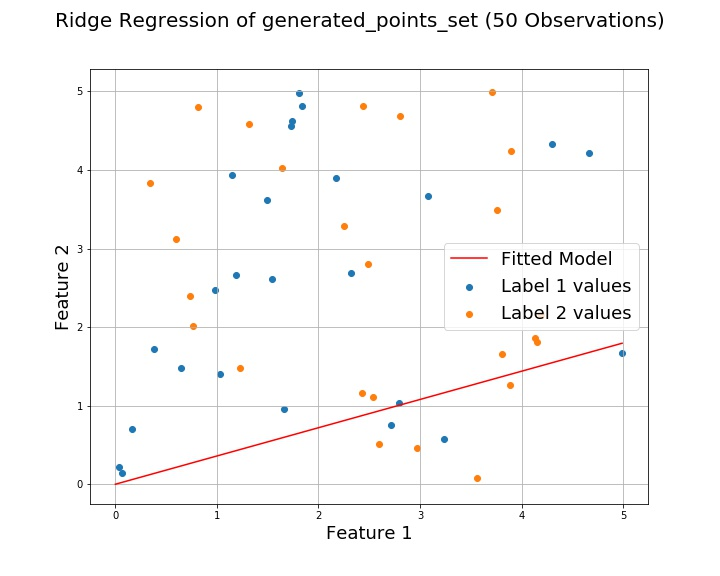
\includegraphics[width=8cm]{ridge_reg_1d_generated_points_set} 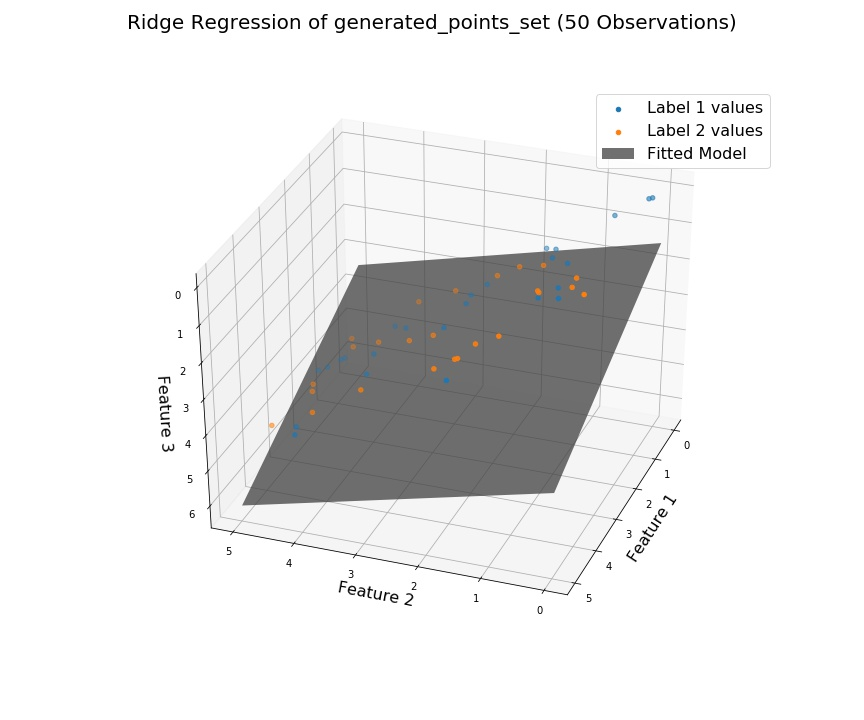
\includegraphics[width=9cm]{ridge_reg_2d_generated_points_set} When comparing the two regression models together, the line of best fit does not appear to change in slope value, at least visually, meaning that a change in regression paramters does not effect the response variable \textit{Y}.

As for the lasso regression model, which is $$\textit{A} = (\textit{y}\textbf{x}' - \frac{\lambda}{2})\textbf{s})(\textbf{x}\textbf{x}')^{-1}$$,using the generated set of points' one-dimensional domain and two-dimensional domain, the plots came out to be 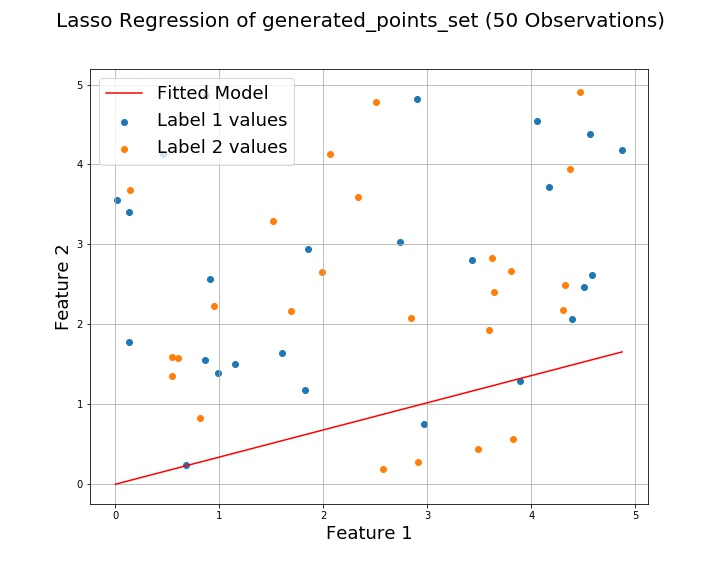
\includegraphics[width=8cm]{lasso_reg_1d_generated_points_set} 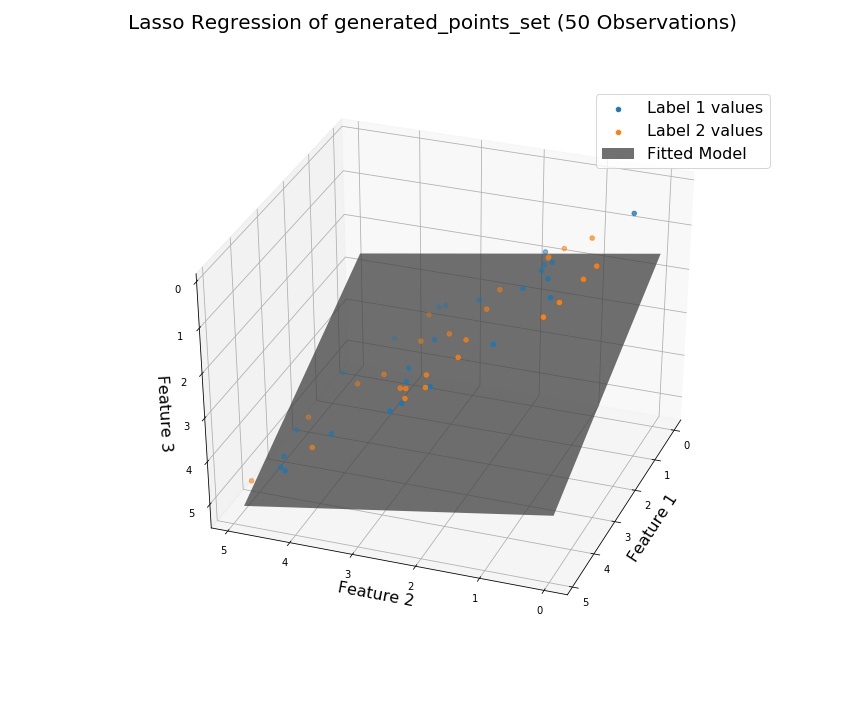
\includegraphics[width=9cm]{lasso_reg_2d_generated_points_set} Notice that still the change in parameters does not visually effect the regression line and regression plane, meaning that adding certain regularization parameters to the error factor does not affect the model.

Finally, the last regression model in the optimization process is the elastic-net regression technique. Elastic-net regression uses both regularization parameters (that were previously used in ridge and lasso regression) to form the estimate: $$\textit{A} = (\textit{y}\textbf{x}' - \frac{\lambda_{2}}{2})\textbf{s})(\textbf{x}\textbf{x}' +\lambda_{1} \textit{I})^{-1}$$ When the domains formed from the generated set of points are used using this type of modelling, they are visualized as such: 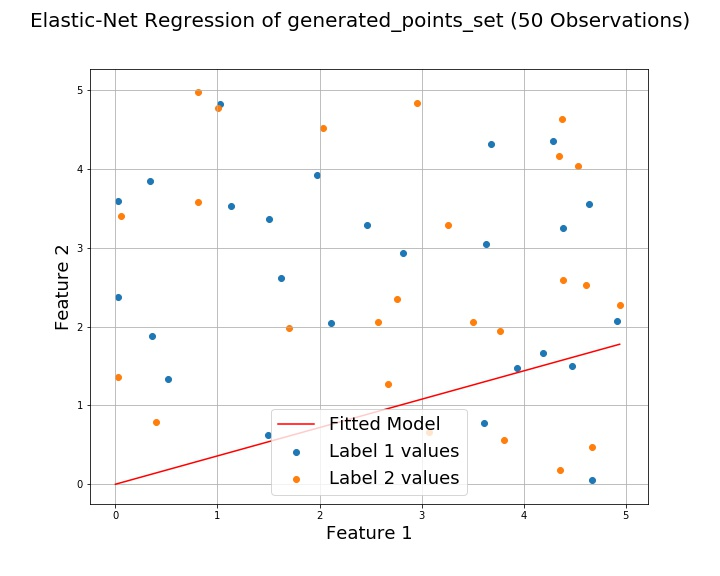
\includegraphics[width=8cm]{en_reg_1d_generated_points_set} 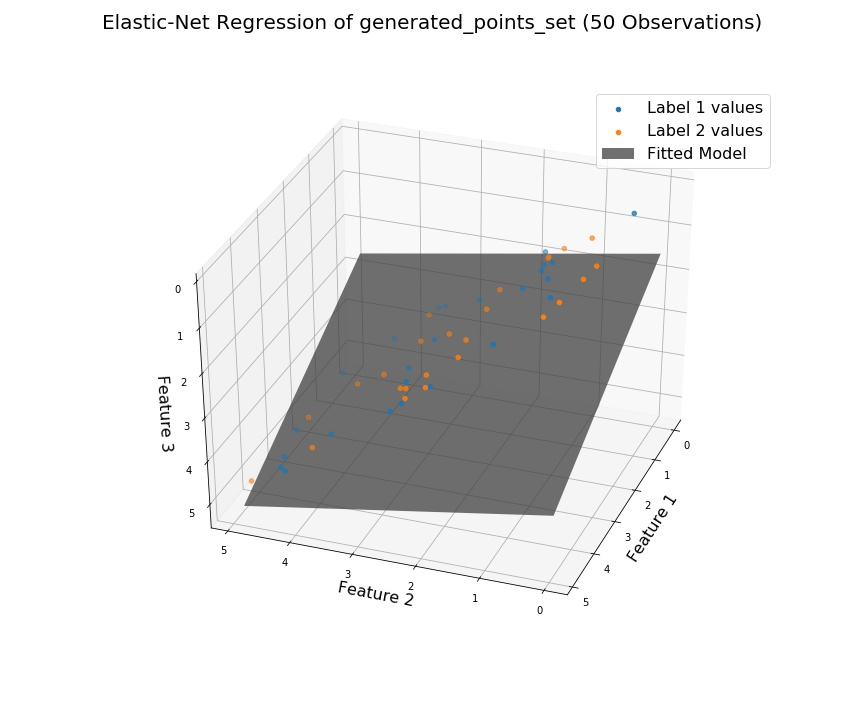
\includegraphics[width=9cm]{en_reg_2d_generated_points_set} Again, there seems to be no distinguishable difference in graphic visualizations. This means that the generated set of points has an optimized model regardless of whatever type of regression would be used on the dataset.

\subsection{Graduate Student Datasets}
\label{grad}

Using the same type of parameters used in standard and ridge regression, the dataset containing information about recent graduate students resulted in the following plots featuring the line of best fit. 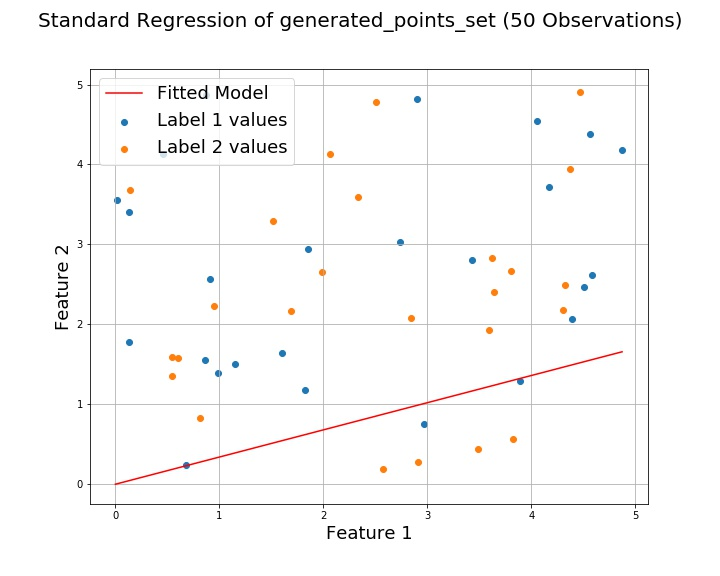
\includegraphics[width=8cm]{std_reg_1d_generated_points_set} 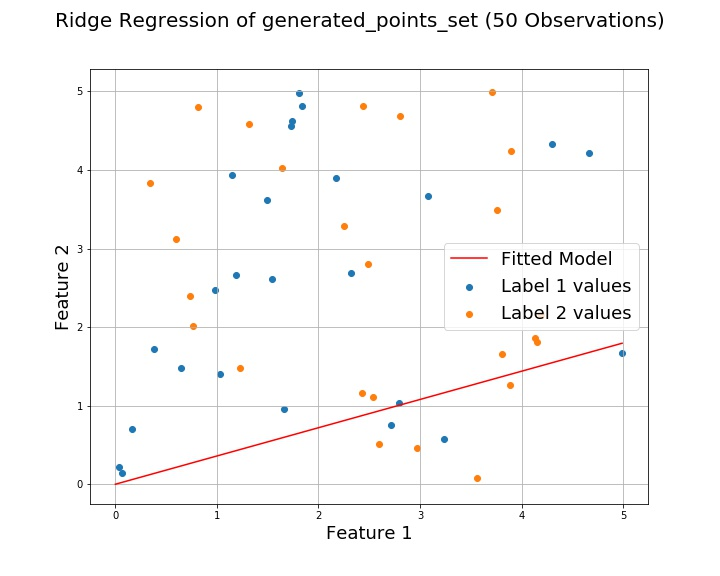
\includegraphics[width=8cm]{ridge_reg_1d_generated_points_set} Unlike the standard and ridge regression models of the generated set of points, there is a noticeable change between both visualizations; the difference being the change in slope for the line of best. In the ridge regression analysis, the model apparently decreases in slope and seems to 

\end{document}